\documentclass[border=4pt]{standalone}
% Shared typography and colours for the standalone figures.
\usepackage{unicode-math}
\setmainfont{TeX Gyre Termes}
\setmathfont{TeX Gyre Termes Math}
\usepackage{tikz}
\usetikzlibrary{arrows.meta,positioning,calc,decorations.pathreplacing}
\usepackage{pgfplots}
\pgfplotsset{compat=1.18}

% One colour per element or subsystem. Record the mapping in
% the working repository conventions and use it identically in every figure.
\definecolor{elemA}{HTML}{1F5FA8}
\definecolor{elemB}{HTML}{B8461B}
\definecolor{elemC}{HTML}{2E7D32}
\definecolor{elemD}{HTML}{6A4C93}
\definecolor{frameline}{HTML}{555555}

% Article-specific diagram styling; common figure-style.tex remains managed.
\usepackage{circuitikz}
\usetikzlibrary{decorations.pathmorphing,fit,backgrounds}
\tikzset{
  every node/.style={font=\small},
  block/.style={draw=frameline,rounded corners=2pt,minimum height=7mm,align=center,fill=white},
  massA/.style={draw=elemA,fill=elemA!10,thick},
  massB/.style={draw=elemB,fill=elemB!10,thick},
  receiver/.style={draw=elemC,fill=elemC!9,thick},
  mediator/.style={draw=elemD,fill=elemD!8,thick},
  flow/.style={-{Latex[length=2.3mm]},thick},
  boundary/.style={draw=frameline,dashed,rounded corners=3pt},
  spring/.style={decorate,decoration={coil,aspect=.4,segment length=3mm,amplitude=1.5mm},thick,elemD}
}

\begin{document}
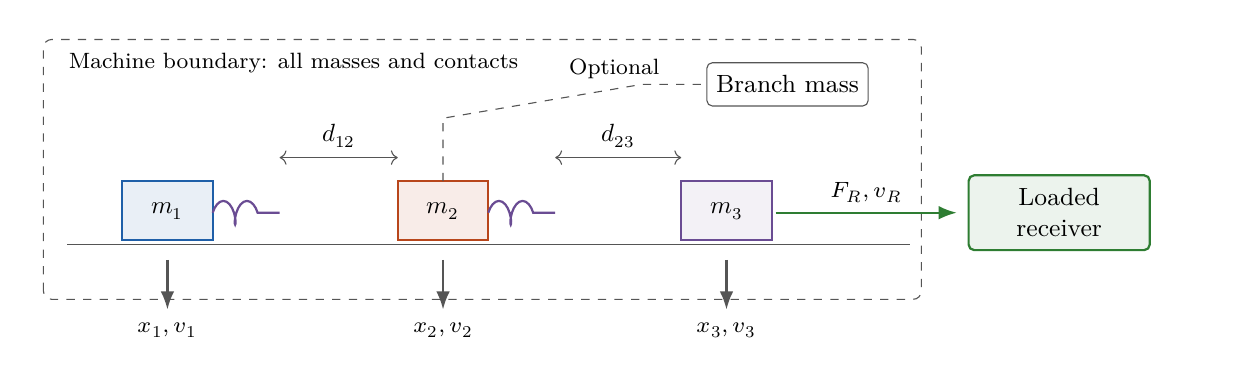
\begin{tikzpicture}
\path[use as bounding box] (0,-.5) rectangle (15,3.55);
\draw[boundary] (.2,.1) rectangle (11.35,3.4);
\node[font=\footnotesize,anchor=north west] at (.4,3.35) {Machine boundary: all masses and contacts};
\draw[frameline] (.5,.8)--(11.2,.8);
\foreach \x/\n/\sty in {1.2/1/massA,4.7/2/massB,8.3/3/mediator} {
 \draw[\sty] (\x,.85) rectangle +(1.15,.75);
 \node at (\x+.575,1.225) {$m_\n$};
 \draw[flow,frameline] (\x+.575,.6)--(\x+.575,-.03);
 \node[font=\footnotesize,below] at (\x+.575,-.07) {$x_\n,v_\n$};
}
\draw[spring] (2.35,1.2)--(3.2,1.2);
\draw[spring] (5.85,1.2)--(6.7,1.2);
\draw[<->,frameline] (3.2,1.9)--(4.7,1.9);
\draw[<->,frameline] (6.7,1.9)--(8.3,1.9);
\node[above] at (3.95,1.9) {$d_{12}$};
\node[above] at (7.5,1.9) {$d_{23}$};
\node[block,minimum width=1.5cm,minimum height=.55cm] (branch) at (9.65,2.83) {Branch mass};
\draw[dashed,frameline] (5.275,1.6)--(5.275,2.4)--(7.8,2.83)--(branch.west);
\node[font=\footnotesize,above] at (7.45,2.78) {Optional};
\draw[flow,elemC] (9.5,1.2)--(11.8,1.2);
\node[font=\footnotesize,above] at (10.65,1.2) {$F_R,v_R$};
\node[block,receiver,minimum width=2.3cm,minimum height=.95cm] at (13.1,1.2) {Loaded\\receiver};
\end{tikzpicture}
\end{document}
